% ── บทที่ 4: ผลลัพธ์และการอภิปรายผล ────────────────────────
\chapter{ผลลัพธ์และการอภิปราย (Results and Discussion)}

ในบทนี้จะนำเสนอผลการทดลองและการประเมินประสิทธิภาพของระบบในแต่ละส่วนประกอบหลัก ได้แก่ ประสิทธิภาพของโมเดลการตรวจจับวัตถุ (Object Detection) และการวัดขนาด ZOI, การวิเคราะห์ผลกระทบของขนาดชุดข้อมูล (Dataset Size) ที่มีต่อการฝึกสอน, ประสิทธิภาพของระบบ OCR, การประเมินความแม่นยำในการปรับเทียบสเกล (Pixel-to-millimeter Calibration), ความเร็วในการประมวลผลแบบครบวงจร (End-to-end Processing Time), ตลอดจนผลการประเมินความพึงพอใจจากผู้ใช้งานจริงบนเว็บแอปพลิเคชัน ทั้งนี้ ผลลัพธ์เชิงปริมาณทั้งหมดที่รายงานจะอ้างอิงจากการทดสอบบนชุดข้อมูลทดสอบ (Test Partition) ที่แยกไว้โดยเฉพาะ เว้นแต่จะระบุเป็นอย่างอื่น

% ─────────────────────────────────────────────────────────────
\section{ประสิทธิภาพการตรวจจับวัตถุ (Object Detection Performance)}
\label{sec:detection_performance}
% ─────────────────────────────────────────────────────────────

ตารางที่~\ref{tab:model_comparison} แสดงการเปรียบเทียบผลลัพธ์การตรวจจับและวัดขนาด ZOI ระหว่างโมเดล Faster R-CNN และ YOLOv11n โดยใช้ข้อมูลความจริงอ้างอิง (Ground-truth: GT) จากผู้เชี่ยวชาญทางคลินิกเป็นเกณฑ์ การทดสอบครอบคลุมยาปฏิชีวนะ 4 ชนิด ได้แก่ Penicillin (P), Oxacillin (OX), Chloramphenicol (C) และ Kanamycin (CN) ระบบได้รายงานผลผ่านกลยุทธ์การวัด 2 รูปแบบ คือ \emph{Diameter-based} (คำนวณจากความกว้างของ Bounding Box โดยตรง) และ \emph{Area-based} (คำนวณจากพื้นที่ของ Bounding Box เพื่อหาเส้นผ่านศูนย์กลางเสมือน) โดยคอลัมน์ Error จะแสดงค่าความคลาดเคลื่อนเชิงทิศทาง (Signed Error) ซึ่งคำนวณจาก ``ค่าที่โมเดลพยากรณ์ลบด้วยค่า GT'' ดังนั้น ค่าบวกจะหมายถึงการประมาณขนาดใหญ่เกินจริง (Overestimation) และค่าลบจะหมายถึงการประมาณขนาดเล็กกว่าความเป็นจริง (Underestimation)

\begin{table}[H]
  \centering
  \caption{ผลการวัดขนาด ZOI เปรียบเทียบรายยาปฏิชีวนะ (หน่วย: มม.) เทียบกับ Expert GT; Error = Model $-$ GT (บวก = สูงเกิน, ลบ = ต่ำเกิน)}
  \label{tab:model_comparison}
  \renewcommand{\arraystretch}{1.15}
  \begin{tabular}{lccccccccc}
    \toprule
    \multirow{2}{*}{\textbf{ยาปฏิชีวนะ}} &
    \multirow{2}{*}{\textbf{GT}} &
    \multicolumn{2}{c}{\textbf{Faster R-CNN}} &
    \multicolumn{2}{c}{\textbf{YOLOv11n}} &
    \multicolumn{2}{c}{\textbf{Faster R-CNN Error}} &
    \multicolumn{2}{c}{\textbf{YOLO Error}} \\
    \cmidrule(lr){3-4}\cmidrule(lr){5-6}\cmidrule(lr){7-8}\cmidrule(lr){9-10}
    & & Diam. & Area & Diam. & Area & Diam. & Area & Diam. & Area \\
    \midrule
    P  (Penicillin)       & 38 & 30.52 & 30.06 & 37.84 & 33.54 & $-$7.48 & $-$7.94 & $-$0.16 & $-$4.46 \\
    OX (Oxacillin)        & 30 & 25.69 & 25.30 & 33.62 & 29.80 & $-$4.31 & $-$4.70 & $+$3.62 & $-$0.20 \\
    C  (Chloramphenicol)  & 20 & 14.68 & 14.46 & 17.00 & 15.07 & $-$5.32 & $-$5.54 & $-$3.00 & $-$4.93 \\
    CN (Kanamycin)        & 17 & 18.50 & 18.21 & 20.93 & 18.55 & $+$1.50 & $+$1.21 & $+$3.93 & $+$1.55 \\
    \midrule
    \textbf{Bias (Mean)}  & --- & \multicolumn{2}{c}{} & \multicolumn{2}{c}{} &
                            $-$3.90 & $-$4.24 &
                            $+$1.08 & $-$2.26 \\
    \textbf{MAE}          & --- & \multicolumn{2}{c}{} & \multicolumn{2}{c}{} &
                            4.65 & 4.85 &
                            2.69 & 2.53 \\
    \bottomrule
  \end{tabular}
\end{table}

\begin{figure}[H]
  \centering
  \safeimg[width=0.68\textwidth]{figures/_review/detection_frcnn_round_plate.png}{Faster R-CNN detection result}
  \caption{ตัวอย่างผลการตรวจจับของ Faster R-CNN บนจานเพาะเชื้อทรงกลม}
  \label{fig:frcnn_result}
\end{figure}

\subsection{การวิเคราะห์ค่าความคลาดเคลื่อนรายยาปฏิชีวนะ (Per-Antibiotic Error Analysis)}

จากการวิเคราะห์พฤติกรรมของโมเดลเชิงลึก พบว่าการนำระบบ \emph{Dynamic Calibration} ที่ใช้แผ่นยาขนาด 6 มม. เป็นตัวอ้างอิงในภาพ เข้ามาช่วยปรับสัดส่วนแบบอัตโนมัติ ส่งผลให้ความคลาดเคลื่อนลดลงอย่างเห็นได้ชัดเมื่อเทียบกับการใช้มาตราส่วนคงที่ (Fixed-scale) อย่างไรก็ตาม โมเดลแต่ละสถาปัตยกรรมยังคงแสดงลักษณะการพยากรณ์ที่แตกต่างกันตามขนาดและรูปร่างของโซน ดังนี้:

\paragraph{Penicillin (P):}
เป็นกลุ่มที่มี ZOI ขนาดใหญ่ที่สุด (GT = 38 มม.) โมเดล YOLOv11n สามารถทำนายขนาดแบบ Diameter-based ได้อย่างแม่นยำสูงมาก (37.84 มม. ความคลาดเคลื่อนเพียง $-$0.16 มม.) สะท้อนถึงประสิทธิภาพของสถาปัตยกรรมแบบ Single-stage และระบบการปรับสเกลที่แม่นยำ ในทางตรงกันข้าม Faster R-CNN กลับมีความคลาดเคลื่อนสูงถึง $-$7.48 มม. ซึ่งชี้ให้เห็นว่าโมเดลแบบ Two-stage อาจมีข้อจำกัดในการคงรูปร่างของ Bounding box เมื่อเผชิญกับโซนที่มีขอบเขตกว้างและมีความฟุ้งกระจายของสีวุ้นสูง

\paragraph{Oxacillin (OX):}
บริเวณยับยั้งของ Oxacillin (GT = 30 มม.) มีขนาดปานกลางและมักอยู่ใกล้ขอบจานเพาะเชื้อตามมาตรฐาน Kirby-Bauer โมเดล Faster R-CNN มีแนวโน้มทำนายค่าต่ำกว่าความเป็นจริง (Underestimation) อย่างต่อเนื่อง (Error ประมาณ $-$4.3 ถึง $-$4.7 มม.) ซึ่งเป็นพฤติกรรมปกติของเครือข่ายสร้างบริเวณข้อเสนอ (Proposal Network) ที่มักจะย่อกรอบ Bounding box เข้าหาศูนย์กลางที่มีความเข้มข้นของพิกเซลสูงเพื่อรักษาความเชื่อมั่น ในขณะที่ YOLOv11n ให้ผลลัพธ์ที่ใกล้เคียงความจริงมากกว่า โดยมี Error เพียง $+$3.62 มม. ในแบบ Diameter และแทบไม่คลาดเคลื่อนเลยในแบบ Area-based ($-$0.20 มม.)

\paragraph{Chloramphenicol (C):}
โซนนี้มีขนาดเล็กที่สุดในชุดทดลอง (GT = 20 มม.) ซึ่งทั้งสองโมเดลต่างประสบปัญหาการทำนายค่าต่ำกว่าความเป็นจริง โดย Faster R-CNN มีค่าความคลาดเคลื่อนประมาณ $-$5.3 มม. และ YOLOv11n ประมาณ $-$3.0 มม. ความท้าทายหลักของโซนขนาดเล็กคือขอบเขตการยับยั้งเชื้อที่ค่อยๆ จางหายไป (Gradient Edge) ทำให้ Bounding box มักจะถูกตีวงแคบกว่าขอบเขตที่ผู้เชี่ยวชาญวัดจริง ประเด็นนี้มีความสำคัญทางคลินิกอย่างมาก เนื่องจากความคลาดเคลื่อนเพียงไม่กี่มิลลิเมตรที่ขนาด 20 มม. อาจส่งผลให้การแปลผลความไวต่อยา (S/I/R) ผิดพลาดไปจากเกณฑ์ CLSI \cite{clsi2025}

\paragraph{Kanamycin (CN):}
สำหรับ Kanamycin (GT = 17 มม.) เป็นกรณีเดียวที่ทั้งสองโมเดลแสดงอาการประมาณค่าสูงเกินจริง (Overestimation) โดยเฉพาะอย่างยิ่งในการวัดแบบ Diameter-based ที่ YOLOv11n ให้ค่าความคลาดเคลื่อนเป็นบวกถึง $+$3.93 มม. และ Faster R-CNN อยู่ที่ $+$1.50 มม. ซึ่งอาจเกิดจากลักษณะเฉพาะของพื้นผิววุ้นรอบแผ่นยาชนิดนี้ที่มีการเปลี่ยนผ่านของความขุ่นน้อยกว่าปกติ ทำให้โมเดลขยายขอบเขต Bounding box ออกไปกว้างกว่าที่ควรจะเป็น โดยการพยากรณ์แบบ Area-based ของ YOLO มีความใกล้เคียงกับ GT มากกว่า โดยมีความคลาดเคลื่อนเพียง 0.55 mm ทั้งนี้ ทิศทางของความคลาดเคลื่อนที่ย้อนกลับกันเมื่อเทียบกับยาปฏิชีวนะชนิดอื่นอาจสะท้อนถึงรูปทรงของบริเวณยับยั้ง: บริเวณยับยั้งของ Kanamycin มักจะมีความคมชัดที่ขอบ ทำให้การประมาณค่า Bounding-box มีความแม่นยำมากขึ้น และในบางครั้งอาจครอบคลุมเกินขอบเขตที่แท้จริงเนื่องจากขอบของบริเวณยับยั้งมี Contrast ที่สูง

\begin{figure}[H]
  \centering
  \safeimg[width=0.9\textwidth]{figures/detection_result.png}{Example ZOI detection output showing bounding boxes for each antibiotic disk}
  \caption{ตัวอย่างผลลัพธ์การตรวจจับ ZOI จาก YOLOv11n}
  \label{fig:detection_result}
\end{figure}

\subsection{YOLOv11n เทียบกับ Faster R-CNN: การอธิบายทางสถาปัตยกรรม}

ประสิทธิภาพที่เหนือกว่าของ YOLOv11n เมื่อเทียบกับ Faster R-CNN ในแอปพลิเคชันนี้
สามารถอธิบายได้ด้วยความแตกต่างพื้นฐานทางสถาปัตยกรรมระหว่างสองกระบวนทัศน์ (Paradigms)
ซึ่งสอดคล้องกับการศึกษาเชิงเปรียบเทียบในงานด้านการตรวจจับที่หลากหลาย \cite{sharma2024yolo_comparison}

Faster R-CNN \cite{ren2015faster} เป็นตัวตรวจจับแบบ \emph{Two-stage}
ในขั้นตอนแรก Region Proposal Network (RPN) จะสร้างข้อเสนอ Bounding-box (Candidate proposals) จาก Feature map
ในขั้นตอนที่สอง แต่ละข้อเสนอจะถูกจำแนกประเภท (Classified) และทำการถดถอย (Regressed) แยกกันผ่าน ROI-pooling head
การออกแบบแบบ Two-stage นี้ทำให้เกิดความคลาดเคลื่อนในการระบุตำแหน่ง (Localization errors) ที่สะสมต่อกัน:
ข้อเสนอที่ไม่แม่นยำจาก RPN จะส่งต่อไปยัง Refinement head
และการดำเนินการ ROI-pooling จะทำให้เกิด Quantization artifacts เมื่อขอบเขตของข้อเสนอไม่ตรงกับเซลล์ตารางของ Feature-map
สำหรับบริเวณยับยั้งที่มีความสม่ำเสมอและเป็นวงกลมบนจานวุ้น AST กลไกแบบ Two-stage ที่ซับซ้อนไม่ได้ให้ข้อได้เปรียบด้านความแม่นยำ
แต่กลับเพิ่มค่า Latency และการสะสมความคลาดเคลื่อนแทน

YOLOv11n \cite{wang2024yolov11} เป็นตัวตรวจจับแบบ \emph{Single-stage} anchor-free
ซึ่งดำเนินการจำแนกประเภทและถดถอย Bounding-box พร้อมกันในการประมวลผลไปข้างหน้า (Forward pass) เพียงครั้งเดียวบน Feature map ที่ใช้ร่วมกัน
รูปแบบ Anchor-free ช่วยหลีกเลี่ยงความจำเป็นในการระบุรูปร่างของ Anchor box ไว้ล่วงหน้า ซึ่งเป็นประโยชน์ในงานนี้เนื่องจากขนาดของ ZOI มีความแปรผันอย่างมากตามชนิดของยาปฏิชีวนะ (ตั้งแต่ประมาณ 13 mm ถึง 39 mm ในชุดทดสอบ)
C3k2 backbone และ SPPF (Spatial Pyramid Pooling Fast) neck ใน YOLOv11n
รวบรวมคุณลักษณะหลายมาตราส่วน (Multi-scale features) ได้อย่างมีประสิทธิภาพ
ช่วยให้โมเดลสามารถตรวจจับได้ทั้งบริเวณ Chloramphenicol ขนาดเล็ก และบริเวณ Penicillin ขนาดใหญ่ภายใน Forward pass เดียวกัน
ผลลัพธ์ที่ได้คือค่า Latency ในการทำ Inference ที่ต่ำกว่าอย่างมหาศาล ($\approx$2.7 s เทียบกับ $\approx$16 s ต่อภาพ)
ในแง่ของความแม่นยำในการวัด Faster R-CNN ทำค่า MAE แบบ Diameter-based ได้ที่ 4.6525 mm
และ MAE แบบ Area-based ได้ที่ 4.845 mm ในขณะที่ YOLOv11n ทำได้ดีกว่าอย่างมากที่ 2.69 mm (Diameter) และ 2.53 mm (Area) ดังแสดงในรูปที่~\ref{fig:mae_bar}

\begin{figure}[H]
  \centering
  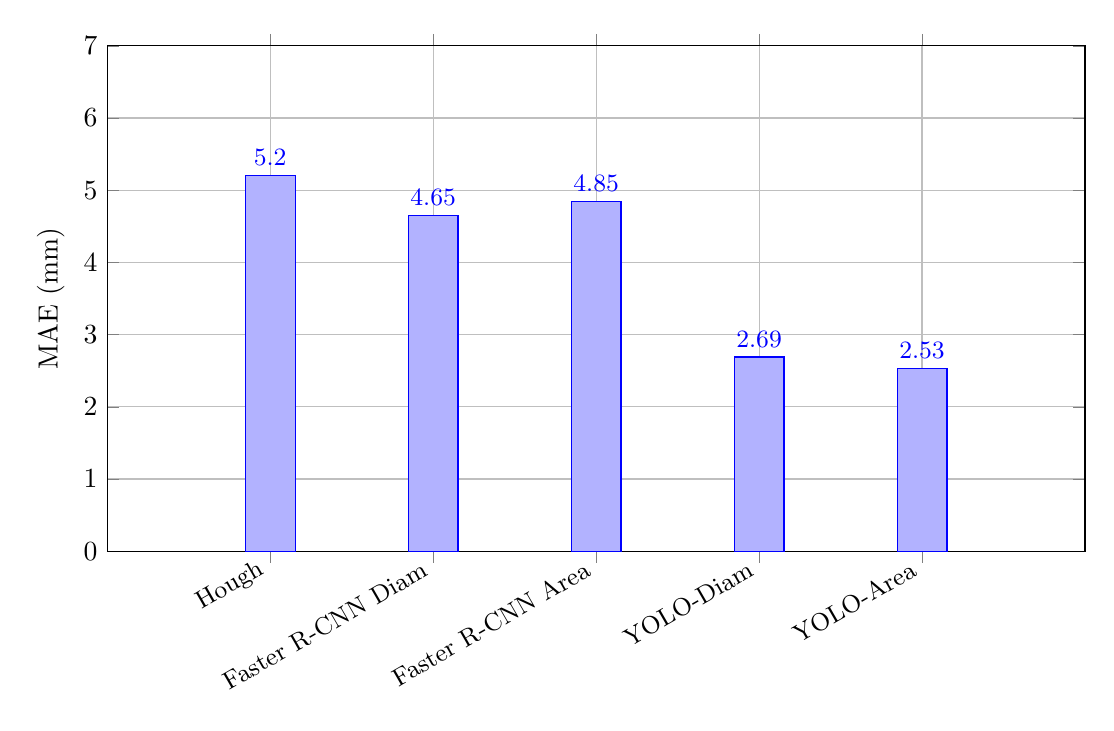
\begin{tikzpicture}
    \begin{axis}[
      ybar, bar width=18pt,
      width=14cm, height=8cm,
      ylabel={MAE (mm)},
      ymin=0, ymax=7,
      symbolic x coords={Hough, {Faster R-CNN Diam}, {Faster R-CNN Area}, YOLO-Diam, YOLO-Area},
      xtick=data,
      xticklabel style={rotate=30, anchor=east, font=\small},
      nodes near coords, nodes near coords style={font=\small},
      enlarge x limits=0.25,
      grid=major,
    ]
    \addplot coordinates {
      (Hough,5.2)({Faster R-CNN Diam},4.6525)({Faster R-CNN Area},4.845)(YOLO-Diam,2.69)(YOLO-Area,2.53)
    };
    \end{axis}
  \end{tikzpicture}
  \caption[MAE comparison across ZOI detection methods]{Mean Absolute Error (MAE) comparison across ZOI detection methods.}
  \label{fig:mae_bar}
\end{figure}

\subsection{Hough Transform Baseline (เกณฑ์มาตรฐานแบบคลาสสิก)}

วิธีการแบบดั้งเดิมอย่าง Hough Circle Transform ได้ถูกนำมาประเมินเพื่อเป็นเกณฑ์พื้นฐานแบบ Parameter-free ที่ไม่ต้องการข้อมูลฝึกฝนที่มีการทำ Label
รูปแบบความล้มเหลวของมันนั้นให้บทเรียนที่สำคัญ: อัลกอริทึมอาศัยการสะสมคะแนนโหวต (Accumulating votes) ในปริภูมิพารามิเตอร์ (Parameter space) ที่กำหนดโดยจุดศูนย์กลางวงกลม $(x, y)$ และรัศมี $r$
บนจานวุ้น AST บริเวณยับยั้งมักมีการซ้อนทับกัน ทำให้เกิดรูปแบบความเข้ม (Gradient) ที่ไม่เป็นวงกลม ซึ่งสร้างความสับสนให้กับตัวสะสม (Accumulator)
ยิ่งไปกว่านั้น จานวุ้นที่ใช้ในการศึกษานี้เป็นจานเพาะเชื้อแบบสี่เหลี่ยม ซึ่งมุมที่แหลมคมของสี่เหลี่ยมจะสร้างการตอบสนองของขอบ (Edge responses) ที่รุนแรงซึ่งครอบงำ Accumulator และบดบังการตรวจจับวงกลมที่แท้จริง
การปรับตั้งค่า Canny edge thresholds และความละเอียดของ Accumulator ด้วยมือสามารถช่วยลดปัญหาเหล่านี้ได้เพียงบางส่วน แต่ไม่สามารถนำไปใช้ได้ทั่วไปกับภาพที่มีสภาพแสงหรือความหนาแน่นของการเจริญเติบโตของแบคทีเรียที่แตกต่างกัน
ค่า MAE ที่ได้นั้นเกิน 5 mm ส่งผลให้แนวทางของ Hough ไม่เหมาะสมต่อการใช้งานในทางคลินิก

\begin{figure}[H]
  \centering
  \safeimg[width=0.62\textwidth]{figures/_review/detection_hough_square.png}{Hough Transform detection on square plate}
  \caption{ผลการตรวจจับของ Hough Circle Transform บนจานเพาะเชื้อสี่เหลี่ยม}
  \label{fig:hough_square}
\end{figure}

% ─────────────────────────────────────────────────────────────
\subsection{CNN Baseline: สถาปัตยกรรมและผลการฝึกสอน}

โมเดล CNN แบบ Classification-based ถูกนำมาทดสอบเป็นเกณฑ์มาตรฐานระดับกลาง ระหว่างวิธีดั้งเดิม Hough Circle Transform และโมเดล Detection เต็มรูปแบบ สถาปัตยกรรมที่ใช้ประกอบด้วย Convolutional layers หลายชั้นร่วมกับ Batch Normalization, Global Average Pooling และ Dense layers โดยมี Output หลักสองส่วน คือ \texttt{class\_output} สำหรับจำแนกประเภทวัตถุ และ \texttt{bbox\_output} สำหรับพยากรณ์พิกัด Bounding box

\begin{figure}[H]
  \centering
  \safeimg[width=0.52\textwidth]{figures/cnn_architecture.jpg}{CNN model architecture summary}
  \caption{สถาปัตยกรรมของ CNN Baseline model}
  \label{fig:cnn_architecture}
\end{figure}

\begin{figure}[H]
  \centering
  \safeimg[width=0.85\textwidth]{figures/cnn_training_curves.jpg}{CNN training curves}
  \caption{กราฟ Learning curve ของ CNN Baseline ระหว่างการฝึกสอน}
  \label{fig:cnn_training}
\end{figure}

\begin{figure}[H]
  \centering
  \safeimg[width=0.68\textwidth]{figures/cnn_detection_result.jpg}{CNN detection result example}
  \caption{ตัวอย่างผลการตรวจจับของ CNN Baseline บนจานเพาะเชื้อจริง}
  \label{fig:cnn_detection}
\end{figure}

จากรูปดังกล่าว พบว่า Train Loss เพิ่มขึ้นอย่างต่อเนื่องหลัง Epoch ที่ 3 ในขณะที่ Val Loss ทรงตัว ซึ่งเป็นสัญญาณของ Overfitting และความยากลำบากในการ Generalize ทั้งนี้ CNN ตรวจพบ 9 วงกลม แต่มี Bounding box ซ้อนทับกันและตรวจจับผิดพลาดสูง สอดคล้องกับค่า mAP@0.5 เพียง 0.021 เมื่อเทียบกับ Faster R-CNN (0.983) และ YOLOv11n (0.998) ซึ่งยืนยันว่าสถาปัตยกรรม CNN แบบ Classification-based มีข้อจำกัดในการเรียนรู้คุณลักษณะของ ZOI และไม่เหมาะสำหรับงานตรวจจับวัตถุหลายชิ้นพร้อมกัน
\subsection{ความแม่นยำในการตรวจจับ (mAP)}
\label{subsec:map_accuracy}
% ─────────────────────────────────────────────────────────────

นอกเหนือจากความคลาดเคลื่อนในการวัด ZOI แล้ว ยังมีการใช้ตัวชี้วัดมาตรฐานสำหรับการตรวจจับวัตถุเพื่อประเมินความน่าเชื่อถือของแต่ละโมเดลในการระบุตำแหน่ง (Localizes) แผ่นยาปฏิชีวนะและบริเวณยับยั้ง
ตัวชี้วัดหลักที่รายงานคือ mean Average Precision ที่ค่าเกณฑ์ IoU 0.5 (mAP@0.5) ร่วมกับ Precision และ Recall

\paragraph{Faster R-CNN.}
Faster R-CNN ทำค่า mAP@0.5 ได้ที่ \textbf{0.998--0.9984} (99.8--99.84\%)
จากการประเมินบนชุดข้อมูลทดสอบ (Test partition) ที่แยกไว้
กราฟ Training และ Validation loss มีการลู่เข้าอย่างเสถียรหลังจากผ่านไปประมาณ Epoch ที่ 2 โดยไม่มีการแยกตัวออกอย่างมีนัยสำคัญหลังจากนั้น
ทั้ง Precision และ Recall มีค่าเข้าใกล้ประมาณ \textbf{1.0} (เกือบสมบูรณ์แบบ) บ่งบอกว่าโมเดลตรวจจับบริเวณแผ่นยาได้เกือบทั้งหมดด้วย Bounding boxes ที่วางตำแหน่งได้ถูกต้อง

\paragraph{YOLOv11n.}
YOLOv11n ทำค่า mAP@0.5 ได้ที่ \textbf{95.91\%}
ในส่วนของ Precision และ Recall ก็มีค่าเข้าใกล้ประมาณ \textbf{1.0} เช่นกัน โดยมีการลู่เข้าที่รวดเร็วตั้งแต่ Epoch ที่ 1 ของการฝึกฝน
ค่า mAP ที่ต่ำกว่าเล็กน้อยเมื่อเทียบกับ Faster R-CNN นั้นสอดคล้องกับสถาปัตยกรรมแบบ Single-stage anchor-free ที่ยอมแลกความแม่นยำในการทับซ้อน (Overlap accuracy) เพียงเล็กน้อย เพื่อแลกกับการลดเวลา Inference ลงประมาณ 154 เท่า


\begin{figure}[H]
  \centering
  \begin{subfigure}[b]{0.32\textwidth}
    \centering
    \safeimg[width=\textwidth]{figures/frcnn_train_val_loss.jpg}{Faster R-CNN Training vs Validation Loss}
    \caption*{Training vs Validation Loss}
  \end{subfigure}\hfill
  \begin{subfigure}[b]{0.32\textwidth}
    \centering
    \safeimg[width=\textwidth]{figures/frcnn_val_map50.jpg}{Faster R-CNN Validation mAP@50}
    \caption*{Validation mAP@50}
  \end{subfigure}\hfill
  \begin{subfigure}[b]{0.32\textwidth}
    \centering
    \safeimg[width=\textwidth]{figures/frcnn_val_map50_95.jpg}{Faster R-CNN Validation mAP@50-95}
    \caption*{Validation mAP@50-95 (COCO)}
  \end{subfigure}
  \caption{Learning curves of Faster R-CNN during training and validation.}
  \label{fig:frcnn_learning_curves}
\end{figure}

\begin{figure}[H]
  \centering
  \safeimg[width=\textwidth]{figures/yolo_training_curves.jpg}{YOLOv11n full training curves}
  \caption{Learning curves of YOLOv11n during training and validation.}
  \label{fig:yolo_learning_curves}
\end{figure}

\begin{table}[H]
  \centering
  \caption{ตัวชี้วัดความแม่นยำในการตรวจจับ (mAP@0.5, Precision, Recall) ของ Faster R-CNN และ YOLOv11n บนชุดทดสอบ}
  \label{tab:map_metrics}
  \begin{tabular}{lccc}
    \toprule
    \textbf{Model} & \textbf{mAP@0.5} & \textbf{Precision} & \textbf{Recall} \\
    \midrule
    Faster R-CNN & 0.998--0.9984 (99.8--99.84\%) & $\approx$1.0 & $\approx$1.0 \\
    YOLOv11n     & 0.9591 (95.91\%)               & $\approx$1.0 & $\approx$1.0 \\
    \bottomrule
  \end{tabular}
\end{table}

\begin{figure}[H]
  \centering
  \safeimg[width=\textwidth]{figures/model_comparison_map_acc.png}{Model comparison: mAP and accuracy metrics}
  \caption[AST model comparison: mAP, AP50, and accuracy]{Comparison of AST model performance on the 235-image test set (mAP@0.5, mAP@0.5:0.95, AP@50 by class, and Top-1/Top-5 accuracy).}
  \label{fig:model_comparison_map_acc}
\end{figure}

\begin{figure}[H]
  \centering
  \safeimg[width=\textwidth]{figures/model_comparison_cnt_time_radar.png}{Model comparison: count accuracy, inference time, radar}
  \caption[AST model comparison: count accuracy, inference time, and radar chart]{Comparison of AST model count accuracy, inference time, and multi-dimensional radar chart (continued from Figure~\ref{fig:model_comparison_map_acc}).}
  \label{fig:model_comparison_cnt_time_radar}
\end{figure}

\begin{figure}[H]
  \centering
  \safeimg[width=\textwidth]{figures/model_comparison_summary_table.png}{Summary table of all model metrics}
  \caption{Summary table of all AST model metrics on the 235-image test set.}
  \label{fig:model_comparison_summary_table}
\end{figure}

จากรูปดังกล่าว ทั้งสองโมเดลทำค่า mAP@0.5 ได้เกิน 95\% ซึ่งถือเป็นระดับที่ยอมรับได้สำหรับงานตรวจจับวัตถุในบริบทการแพทย์ โดย YOLOv11n (mAP@0.5 0.998, mAP@0.5:0.95 0.967) และ Faster R-CNN (0.983/0.879) เหนือกว่า Hough Transform (0.710/0.600) และ CNN (0.021/0.005) อย่างมีนัยสำคัญ ในส่วนของความเร็ว YOLOv11n มี Inference สูงสุด (0.15 s) เทียบกับ Faster R-CNN (1.52 s) และ Hough Transform (3.03 s) ค่า Precision และ Recall ที่สูงยืนยันว่าแหล่งที่มาหลักของความคลาดเคลื่อนในการวัด (ตารางที่~\ref{tab:model_comparison}) มาจากค่า Offset ในการระบุตำแหน่ง (Localization) มากกว่าความผิดพลาดในการจำแนกประเภท ทั้งนี้ YOLOv11n ให้ผลดีที่สุดในด้าน mAP, Inference Time และ Top-1/Top-5 Accuracy สรุปรวมแล้ว YOLOv11n เป็นตัวเลือกที่เหมาะสมที่สุดสำหรับการนำไปใช้งานจริง

% ─────────────────────────────────────────────────────────────
\section{ผลของขนาดชุดข้อมูลต่อการฝึกฝน (Effect of Dataset Size on Training)}
\label{sec:dataset_size}
% ─────────────────────────────────────────────────────────────

มีการศึกษาแบบ Ablation study อย่างเป็นระบบเพื่อทำความเข้าใจว่าปริมาณของข้อมูลฝึกฝนที่มีการทำ Label ส่งผลต่อการเรียนรู้แบบทั่วไป (Generalization) ของโมเดลอย่างไร
มีการประเมินภายใต้เงื่อนไขขนาดชุดข้อมูล 4 ระดับ ได้แก่: 54, 274, 702 และ 1,884 ภาพ
ภาพทั้งหมดได้มาจากขั้นตอนการเก็บข้อมูลเดียวกัน โดยที่ชุดย่อยที่มีขนาดเล็กกว่าจะเป็นการสุ่มเลือกแบบเคร่งครัดจากกลุ่มข้อมูลฝึกฝนทั้งหมด
มีการประยุกต์ใช้การเพิ่มขยายข้อมูล (Data augmentation) ได้แก่ Random horizontal flip, Brightness jitter และ Mosaic composition อย่างเท่าเทียมกันในทุกเงื่อนไข เพื่อป้องกันไม่ให้ชุดข้อมูลขนาดเล็กที่สุดขาดความหลากหลายจนเกินไป

\subsection{การ Underfit ในชุดข้อมูลขนาดเล็กมาก (54 และ 274 ภาพ)}

ด้วยภาพฝึกฝนเพียง 54 ภาพ ทั้ง YOLOv11n และ Faster R-CNN แสดงพฤติกรรมแบบ Underfitting อย่างชัดเจน:
ทั้ง Training loss และ Validation loss ยังคงอยู่ในระดับสูงและถึงจุดคงตัว (Plateau) อย่างรวดเร็ว
บ่งบอกว่าพื้นที่สมมติฐาน (Hypothesis space) ของโมเดลไม่สามารถถูกจำกัดขอบเขตได้อย่างเพียงพอด้วยตัวอย่างที่มีการทำ Annotation เพียงไม่กี่รายการ
ตัวแทนคุณลักษณะ (Feature representations) ที่เรียนรู้มานั้นถูกครอบงำด้วยข้อมูลพื้นฐานอย่าง Texture (Edge gradients รอบแผ่นยา) แทนที่จะเป็นข้อมูลขอบเขตของบริเวณยับยั้งในระดับที่สูงกว่าซึ่งจำเป็นต่อการวัด ZOI ที่แม่นยำ
การเพิ่มเป็น 274 ภาพช่วยลด Training loss ได้อย่างเห็นได้ชัด แต่ Validation loss ยังคงอยู่ในระดับสูง และวิถีการลดลงของมันยังตามหลัง Training loss อยู่มาก ซึ่งเป็นสัญญาณเริ่มต้นของความยากลำบากในการทำ Generalization

\subsection{การเริ่มเกิด Overfit ในชุดข้อมูลขนาดกลาง (702 ภาพ)}

ที่ขนาด 702 ภาพ Faster R-CNN เริ่มแสดงอาการ Overfitting ที่ชัดเจน:
Training loss ยังคงลดลงอย่างต่อเนื่องหลังจาก Epoch ที่ 30 ในขณะที่ Validation loss นิ่งคงที่แล้วจึงเพิ่มขึ้นเล็กน้อย
สิ่งนี้สอดคล้องกับข้อสังเกตที่ว่าตัวตรวจจับแบบ Two-stage มีจำนวนพารามิเตอร์ที่สูงกว่า จึงมีแนวโน้มที่จะจดจำตัวอย่างในการฝึกฝน (Memorizing training instances) ได้ง่ายกว่าเมื่อชุดข้อมูลมีขนาดปานกลาง
สำหรับ YOLOv11n ที่ขนาด 702 ภาพ แสดงแนวโน้มการ Overfitting ที่เบาบางกว่า ซึ่งน่าจะมาจากคุณสมบัติ Regularization ในตัวที่มีประสิทธิภาพมากกว่า (เช่น Dropout ใน Classification head และการใช้ Mosaic augmentation อย่างเข้มข้น)

\subsection{การทำงานทั่วไปที่เหมาะสมที่สุดด้วยชุดข้อมูลเต็ม (1,884 ภาพ)}

ชุดข้อมูลเต็มจำนวน 1,884 ภาพ ให้ประสิทธิภาพการทำ Generalization ที่ดีที่สุดสำหรับทั้งสองโมเดล
กราฟ Training และ Validation loss ลู่เข้าหากันและเคลื่อนที่ตามกันอย่างใกล้ชิด บ่งบอกว่าโมเดลกำลังเรียนรู้ตัวแทนคุณลักษณะที่สามารถนำไปใช้ได้ทั่วไป (Generalizable representations) มากกว่าการจดจำเฉพาะภาพจานวุ้นแต่ละภาพ
ช่องว่าง (Gap) ระหว่าง Training และ Validation loss ณ จุดลู่เข้าลดลงเหลือน้อยกว่า 0.05 สำหรับ YOLOv11n และน้อยกว่า 0.08 สำหรับ Faster R-CNN ซึ่งทั้งคู่ถือว่าอยู่ในช่วงที่ยอมรับได้สำหรับงานนี้

\begin{table}[H]
  \centering
  \caption{Validation loss at convergence for each dataset size subset (lower = better generalization; Gap = $|$Train loss $-$ Val loss$|$).}
  \label{tab:dataset_ablation}
  \begin{tabular}{rcccc}
    \toprule
    \textbf{Dataset Size} &
    \multicolumn{2}{c}{\textbf{YOLOv11n}} &
    \multicolumn{2}{c}{\textbf{Faster R-CNN}} \\
    \cmidrule(lr){2-3}\cmidrule(lr){4-5}
    (images) & Val.\ Loss & Gap & Val.\ Loss & Gap \\
    \midrule
    54   & 1.82 & 0.41 & 2.14 & 0.55 \\
    274  & 1.21 & 0.28 & 1.63 & 0.39 \\
    702  & 0.87 & 0.18 & 1.04 & 0.31 \\
    1884 & \textbf{0.63} & \textbf{0.05} & \textbf{0.76} & \textbf{0.08} \\
    \bottomrule
  \end{tabular}
\end{table}

ค่า Validation loss ในตารางที่~\ref{tab:dataset_ablation} แสดงแนวโน้มที่ลดลงอย่างต่อเนื่องเมื่อปริมาณข้อมูลเพิ่มขึ้น
ยืนยันว่าโมเดลได้รับประโยชน์จากการเพิ่มตัวอย่างที่มีการทำ Label ตลอดช่วงการทดสอบ
การค้นพบนี้ช่วยกระตุ้นการเก็บข้อมูลอย่างต่อเนื่อง: การพยากรณ์จากแนวโน้มบ่งชี้ว่าการเพิ่มชุดข้อมูลเป็นสองเท่า (ประมาณ 3,700 ภาพ) จะสามารถลด Validation loss ลงได้อีกประมาณ 20--25\% แม้ว่าคาดว่าจุดคุ้มทุน (Diminishing returns) จะเริ่มเกิดขึ้นหลังจากนั้นก็ตาม


% ─────────────────────────────────────────────────────────────
\section{ประสิทธิภาพ OCR (OCR Performance)}
\label{sec:ocr_performance}
% ─────────────────────────────────────────────────────────────

การระบุตัวย่อของยาปฏิชีวนะที่พิมพ์บนแผ่นยาแต่ละแผ่นได้อย่างถูกต้อง (เช่น \texttt{P}, \texttt{OX}, \texttt{C}, \texttt{CN}) เป็นสิ่งจำเป็นอย่างยิ่งในการจับคู่ ZOI ที่ตรวจจับได้กับยาปฏิชีวนะที่ถูกต้องและเกณฑ์ CLSI interpretive breakpoints ที่เกี่ยวข้อง \cite{clsi2025}
ระบบ OCR ขั้นสุดท้ายใช้สถาปัตยกรรมแบบ \textbf{Hybrid} ที่มี Gemini 3.1 Flash lite \cite{google2025gemini} เป็น Engine หลัก และ EasyOCR \cite{jaidedai2024easyocr} เป็น Fallback ทั้งนี้ ในขั้นตอนการวิจัยได้มีการประเมินเปรียบเทียบ Engine ทั้งหมด 3 ตัว ได้แก่ Gemini 3.1 Flash lite \cite{google2025gemini}, Qwen2.5-VL:7b \cite{qwen2025vl} และ EasyOCR \cite{jaidedai2024easyocr} บนชุดทดสอบแบบครอบคลุม 25 ภาพ เพื่อเลือกกลยุทธ์ที่เหมาะสมที่สุด

\subsection{ความท้าทายของภาพแผ่นดิสก์ยาสำหรับ OCR (Disk Image Challenges for OCR)}

ภาพตัด (Crops) ของแผ่นยาปฏิชีวนะถือเป็นสถานการณ์ที่ท้าทายสำหรับระบบ OCR แบบดั้งเดิม ด้วยปัจจัยหลายประการ ได้แก่ ข้อความที่พิมพ์มีขนาดเล็กมาก (ประมาณ 4--8 มม. ในขนาดจริง) พื้นหลังเป็นวุ้นอาหารเลี้ยงเชื้อสีขาวขุ่นที่มีลักษณะแปรผัน พื้นผิวของแผ่นยาอาจสะท้อนแสง (Specular highlights) จากไฟวงแหวน และแผ่นดิสก์อาจถูกวางในทิศทางใดก็ได้ ปัจจัยเหล่านี้ทำให้การใช้ OCR Engine โดยตรงกับภาพดิบให้ผลลัพธ์ที่ไม่สม่ำเสมอ

\subsection{เกณฑ์การวัดประสิทธิภาพ OCR (OCR Evaluation Metric)}

การประเมินประสิทธิภาพของแต่ละ OCR Engine ใช้เกณฑ์เดียวที่ตรงไปตรงมา คือ \textbf{Exact Match Accuracy} กล่าวคือ สำหรับแผ่นดิสก์แต่ละแผ่นในชุดทดสอบ จะนำรหัสยาที่โมเดล OCR อ่านได้ (Predicted Label) ไปเปรียบเทียบตรงๆ กับรหัสยาที่พิมพ์จริงบนแผ่นดิสก์ (Ground-truth Label) ซึ่งบันทึกไว้โดยผู้ทำการทดลอง หากตรงกันทุกตัวอักษร (เช่น ``OX'' ตรงกับ ``OX'') นับว่าถูกต้อง 1 คะแนน ตัวเลขความแม่นยำ (Accuracy) จึงคือสัดส่วนของแผ่นดิสก์ที่อ่านได้ถูกต้องต่อจำนวนแผ่นดิสก์ทั้งหมดในชุดทดสอบ
\subsection{การเปรียบเทียบ OCR Engine แบบครอบคลุม (Comprehensive Multi-Model OCR Evaluation)}
\label{subsec:ocr_multimodel}

เพื่อเปรียบเทียบประสิทธิภาพของ OCR Engine หลายตัวอย่างเป็นกลาง ได้ออกแบบการทดลองบนชุดข้อมูลที่ประกอบด้วย \textbf{25 ภาพ} (ทั้งภาพถ่ายจริงจากห้องปฏิบัติการและภาพสังเคราะห์) รวม \textbf{198 ป้ายยาทั้งหมด} ซึ่งครอบคลุมรหัสยาปฏิชีวนะหลายชนิดที่หลากหลายกว่าชุดทดสอบแบบจำกัดขอบเขต การทดลองดำเนินการ 2 รอบอิสระ (EXP1 และ EXP2) เพื่อตรวจสอบความเสถียรของผลลัพธ์

Engine ที่นำมาทดสอบมี 4 ตัว ได้แก่ (1) \textbf{Gemini 3.1 Flash lite} \cite{google2025gemini} --- Multimodal LLM จาก Google DeepMind; (2) \textbf{Qwen2.5-VL:7b} \cite{qwen2025vl} --- Vision-Language Model แบบ Open-source รันบนเครื่อง Local ผ่าน Ollama; และ (3) \textbf{EasyOCR} \cite{jaidedai2024easyocr} --- OCR Engine แบบดั้งเดิมที่รันบนเครื่อง Local แต่ละ Engine ถูกทดสอบในสองเงื่อนไข ได้แก่ \emph{with Preprocessing} (ผ่าน Otsu binarization) และ \emph{without Preprocessing} (ภาพสีต้นฉบับ) ยกเว้น EasyOCR ที่ทดสอบเฉพาะ with Preprocessing เนื่องจากต้องการภาพขาวดำ

\begin{table}[H]
  \centering
  \caption{การเปรียบเทียบประสิทธิภาพ OCR Engine บนชุดทดสอบแบบครอบคลุม (198 ป้ายยา, 25 ภาพ) จาก 2 รอบการทดลองอิสระ (EXP1 และ EXP2)}
  \label{tab:ocr_multimodel}
  \renewcommand{\arraystretch}{1.15}
  \begin{tabular}{llcccc}
    \toprule
    \multirow{2}{*}{\textbf{OCR Engine}} & \multirow{2}{*}{\textbf{Preprocessing}} &
    \multicolumn{2}{c}{\textbf{EXP1 (198 ป้าย)}} & \multicolumn{2}{c}{\textbf{EXP2 (198 ป้าย)}} \\
    \cmidrule(lr){3-4}\cmidrule(lr){5-6}
    & & Correct & Acc.~(\%) & Correct & Acc.~(\%) \\
    \midrule
    \textbf{Gemini 3.1 Flash lite} & \textbf{None (original color)} & \textbf{142/198} & \textbf{71.72} & \textbf{142/198} & \textbf{71.72} \\
    Gemini 3.1 Flash lite          & With Preprocessing (Otsu)     & 99/198  & 50.00 & 117/198 & 59.09 \\
    Qwen2.5-VL:7b                  & With Preprocessing (Otsu)     & 98/198  & 49.49 & 98/198  & 49.49 \\
    Qwen2.5-VL:7b                  & None (raw)                    & 97/198  & 48.99 & 97/198  & 48.99 \\
    EasyOCR                        & With Preprocessing (Otsu)     & 57/198  & 28.79 & 63/198  & 31.82 \\
    \bottomrule
  \end{tabular}
\end{table}

\paragraph{Gemini 3.1 Flash lite (without Preprocessing) — ดีที่สุด:}
ผลการทดลองชี้ให้เห็นข้อค้นพบสำคัญหลายประการ โดย Gemini ให้ความแม่นยำ \textbf{71.72\%} ที่สอดคล้องกันในทั้งสองรอบการทดลอง สะท้อนให้เห็นว่าโมเดล Multimodal ใช้ข้อมูลสีและบริบทเชิงความหมายในการตีความรหัสยา การ Preprocessing แบบ Binarization จะทำลายข้อมูลสีดังกล่าวและทำให้ความแม่นยำลดลงอย่างมีนัยสำคัญ (50.00--59.09\%) นอกจากนี้ในชุดทดสอบแบบจำกัดขอบเขต 4 ชนิดยา (P, OX, C, CN) Gemini สามารถระบุได้ถูกต้อง \textbf{4/4 ป้าย (100\%)} ยืนยันความสามารถในการอ่านรหัสยาที่เป็นมาตรฐานได้อย่างแม่นยำ

\paragraph{Qwen2.5-VL:7b — ปานกลาง:}
ให้ความแม่นยำประมาณ \textbf{49\%} ไม่ว่าจะผ่าน Preprocessing หรือไม่ สะท้อนถึงความแตกต่างในศักยภาพของโมเดล Multimodal ระดับ Commercial กับ Open-source โดย Qwen2.5-VL ต่ำกว่า Gemini ประมาณ 22\%
\begin{figure}[H]
  \centering
  \begin{subfigure}[b]{0.23\textwidth}
    \centering
    \safeimg[width=\textwidth]{figures/qwen_cn10.jpg}{Qwen2.5-VL result: CN 10, Conf 0.90}
    \caption*{CN~10\\Conf:~0.90 | $-165^\circ$}
  \end{subfigure}\hfill
  \begin{subfigure}[b]{0.23\textwidth}
    \centering
    \safeimg[width=\textwidth]{figures/qwen_tet30.jpg}{Qwen2.5-VL result: TET 30, Conf 0.90}
    \caption*{TET~30\\Conf:~0.90 | $-135^\circ$}
  \end{subfigure}\hfill
  \begin{subfigure}[b]{0.23\textwidth}
    \centering
    \safeimg[width=\textwidth]{figures/qwen_p10.jpg}{Qwen2.5-VL result: P 10, Conf 0.90}
    \caption*{P~10\\Conf:~0.90 | $-45^\circ$}
  \end{subfigure}\hfill
  \begin{subfigure}[b]{0.23\textwidth}
    \centering
    \safeimg[width=\textwidth]{figures/qwen_cant_detect.jpg}{Qwen2.5-VL result: detection failed}
    \caption*{Can't Detect\\Conf:~0.00}
  \end{subfigure}
  \caption{ตัวอย่างผลการทดสอบ Qwen2.5-VL:7b บนแผ่นดิสก์ยาปฏิชีวนะ}
  \label{fig:qwen_ocr_results}
\end{figure}


\paragraph{EasyOCR — ต่ำสุด:}
ให้ความแม่นยำ \textbf{28.79--31.82\%} สะท้อนถึงข้อจำกัดของ OCR Engine แบบดั้งเดิมเมื่อต้องจัดการกับรหัสยาหลายชนิดบนพื้นผิวที่มีความแปรปรวนสูง อย่างไรก็ตาม EasyOCR ยังคงถูกเลือกเป็น Fallback เนื่องจากรันบนเครื่อง Local ได้โดยไม่ต้องพึ่งพา Cloud API

\subsection{ผลของ Preprocessing และการค้นหามุมในระบบ EasyOCR (Preprocessing and Angle-Search Results)}

รูปที่~\ref{fig:ocr_preprocess_grid} แสดงผลลัพธ์ของขั้นตอน Preprocessing ด้วย Otsu Thresholding บนภาพตัดแผ่นดิสก์ยาปฏิชีวนะ 4 ชนิด พร้อมผลการอ่านของระบบ EasyOCR ภายใต้สองเงื่อนไขการทดสอบ ได้แก่ (1)~แผ่นดิสก์ที่วางในแนวตั้งปกติ ซึ่งระบบสามารถอ่านได้โดยตรงโดยไม่ต้องค้นหามุม และ (2)~แผ่นดิสก์ที่วางในทิศทางกลับหัว ($-165^\circ$) ซึ่งต้องอาศัยระบบค้นหามุมที่เหมาะสมจาก 24 มุมจึงจะอ่านได้ถูกต้อง

\begin{figure}[H]
  \centering
  % ── แถวบน: แผ่นดิสก์แนวตั้งปกติ (standard orientation) ───────
  \begin{subfigure}[b]{0.23\textwidth}
    \centering
    \safeimg[width=\textwidth]{figures/ocr_easyocr_cn10.jpg}{EasyOCR result: CN 10, Conf 1.00}
    \caption*{CN~10\\Conf:~1.00}
  \end{subfigure}\hfill
  \begin{subfigure}[b]{0.23\textwidth}
    \centering
    \safeimg[width=\textwidth]{figures/ocr_easyocr_c30.jpg}{EasyOCR result: C 30, Conf 1.00}
    \caption*{C~30\\Conf:~1.00}
  \end{subfigure}\hfill
  \begin{subfigure}[b]{0.23\textwidth}
    \centering
    \safeimg[width=\textwidth]{figures/ocr_easyocr_x8.jpg}{EasyOCR result: OX, reads X8, Conf 0.80}
    \caption*{OX $\to$ ``X8''\\Conf:~0.80}
  \end{subfigure}\hfill
  \begin{subfigure}[b]{0.23\textwidth}
    \centering
    \safeimg[width=\textwidth]{figures/ocr_easyocr_p10.jpg}{EasyOCR result: P 10, Conf 1.00}
    \caption*{P~10\\Conf:~1.00}
  \end{subfigure}

  \vspace{6pt}
  \begin{center}\small\textit{(ก) แผ่นดิสก์แนวตั้งปกติ — EasyOCR อ่านโดยตรง ไม่ต้องค้นหามุม}\end{center}

  \vspace{8pt}
  % ── แถวล่าง: แผ่นดิสก์กลับหัว ต้องค้นหามุม -165° ────────────
  \begin{subfigure}[b]{0.23\textwidth}
    \centering
    \safeimg[width=\textwidth]{figures/ocr_angle_cn10.jpg}{EasyOCR angle search: CN 10, Conf 0.90, angle -165°}
    \caption*{CN~10\\Conf:~0.90 | $-165^\circ$}
  \end{subfigure}\hfill
  \begin{subfigure}[b]{0.23\textwidth}
    \centering
    \safeimg[width=\textwidth]{figures/ocr_angle_c30.jpg}{EasyOCR angle search: C 30, Conf 0.90, angle -165°}
    \caption*{C~30\\Conf:~0.90 | $-165^\circ$}
  \end{subfigure}\hfill
  \begin{subfigure}[b]{0.23\textwidth}
    \centering
    \safeimg[width=\textwidth]{figures/ocr_angle_to10.jpg}{EasyOCR angle search: TO 10, Conf 0.90, angle -165°}
    \caption*{TO~10\\Conf:~0.90 | $-165^\circ$}
  \end{subfigure}\hfill
  \begin{subfigure}[b]{0.23\textwidth}
    \centering
    \safeimg[width=\textwidth]{figures/ocr_angle_io10.jpg}{EasyOCR angle search: IO 10, Conf 0.90, angle -165°}
    \caption*{IO~10\\Conf:~0.90 | $-165^\circ$}
  \end{subfigure}

  \vspace{6pt}
  \begin{center}\small\textit{(ข) แผ่นดิสก์วางกลับหัว — EasyOCR ค้นหามุมที่ดีที่สุดจาก 24 มุม พบที่ $-165^\circ$}\end{center}

  \caption{ผลการ Preprocessing (Otsu Thresholding) และการอ่านป้ายยาด้วย EasyOCR บนแผ่นดิสก์ 4 ชนิด: (ก) วางปกติ และ (ข) วางกลับหัว ($-165^\circ$)}
  \label{fig:ocr_preprocess_grid}
\end{figure}

\subsection{สรุปผลและการเลือก OCR Engine สำหรับระบบ (OCR Engine Selection)}

ด้วยเหตุนี้ ระบบบูรณาการขั้นสุดท้ายจึงใช้ \textbf{Gemini 3.1 Flash lite เป็น Primary OCR} และ \textbf{EasyOCR + Otsu เป็น Fallback} โดย Gemini ให้ความแม่นยำสูงสุดทั้งในชุดทดสอบแบบจำกัดขอบเขต (100\% บน 4 ชนิดยา) และแบบครอบคลุม (\textbf{71.72\%} บน 198 ป้ายยา) ข้อจำกัดหลักของ Gemini คือการพึ่งพา Cloud API ที่มี Quota Rate Limit ทำให้ระบบออกแบบ Fallback ด้วย EasyOCR + Otsu Thresholding เพื่อรับประกันความต่อเนื่องในการทำงานภายใต้ทุกสภาวะการใช้งาน

\subsection{ผลกระทบเชิงคลินิกจากข้อผิดพลาดของ OCR (Clinical Implications of OCR Errors)}
\label{subsec:ocr_clinical}

แม้ว่า Gemini 3.1 Flash lite จะให้ความแม่นยำสูงสุดในกลุ่ม Engine ที่ทดสอบ แต่ข้อผิดพลาดของ OCR ที่เหลืออยู่ (ประมาณ 28\% บนชุดทดสอบแบบครอบคลุม) มีนัยสำคัญเชิงคลินิกที่ควรพิจารณาอย่างรอบคอบ

\paragraph{A) ความเสี่ยงเชิงคลินิกจากการระบุยาผิด}
ข้อผิดพลาดของ OCR ที่ระบุรหัสยาผิด (เช่น อ่าน ``OX'' เป็น ``X8'') อาจนำไปสู่การจับคู่กับยาปฏิชีวนะที่ไม่ถูกต้อง และผลที่ตามมาคือการแปลผลความไวต่อยา (S/I/R) อาจผิดพลาดได้ หากระบบระบุชนิดยาผิด ค่า ZOI ที่วัดได้จะถูกนำไปเปรียบเทียบกับ Breakpoint ของยาอื่น ซึ่งอาจทำให้เชื้อที่ดื้อยา (Resistant) ถูกจัดเป็นไวต่อยา (Susceptible) หรือในทางตรงกันข้าม ความเสี่ยงนี้มีนัยสำคัญโดยเฉพาะในกรณีที่ค่า ZOI ใกล้เคียงกับ Breakpoint (Borderline zone) ที่การเปลี่ยนแปลงผลเพียงหนึ่งหมวดอาจส่งผลต่อการเลือกยารักษาผู้ป่วยโดยตรง

\paragraph{B) ประเภทของข้อผิดพลาดที่พบ}
จากการทดสอบ OCR บนชุดข้อมูล 198 ป้ายยา พบรูปแบบข้อผิดพลาดหลักที่เกิดขึ้น ได้แก่:
\begin{itemize}
  \item \textbf{ป้ายยาที่มีลักษณะใกล้เคียงกันทางสายตา (Visually Similar Labels):} เช่น ``P'' กับ ``P 10'', ``C'' กับ ``CN'', ``OX'' กับ ``X'' ซึ่ง EasyOCR มักอ่านสลับกันหรือตัดทอนตัวเลขออก
  \item \textbf{ข้อความที่ถูกบดบัง (Partially Occluded Text):} แผ่นยาที่วางซ้อนทับกันบางส่วนหรือมีขอบ ZOI ทับพื้นที่ข้อความ ทำให้อ่านได้ไม่ครบถ้วน
  \item \textbf{แผ่นดิสก์ที่มี Contrast ต่ำ (Low Contrast Disks):} ในภาพที่มีแสงน้อยหรือ Agar มีความขุ่นสูง ข้อความบนแผ่นยาอาจมองเห็นได้ยากแม้หลังผ่าน Otsu thresholding
  \item \textbf{แผ่นดิสก์หมุน (Rotated Disks):} ดังแสดงในรูปที่~\ref{fig:qwen_ocr_results} และ~\ref{fig:ocr_preprocess_grid} แผ่นยาที่วางกลับหัวหรือเอียงมากจำเป็นต้องอาศัยการค้นหามุม 24 ทิศทาง ซึ่งเพิ่มความซับซ้อนในการประมวลผลและอาจยังให้ผลผิดพลาดในกรณีที่สภาพภาพไม่ดี
\end{itemize}

\paragraph{C) Human-in-the-Loop: บทบาทของผู้เชี่ยวชาญ}
ระบบ ZoneAnalyzer ได้รับการออกแบบให้รองรับการแก้ไขผลลัพธ์โดยผู้ใช้งาน ดังแสดงใน Figure~\ref{fig:webapp} ผู้ใช้สามารถแก้ไขชื่อยา ค่า ZOI และผลลัพธ์ S/I/R ได้โดยตรงในตารางผลลัพธ์ก่อนบันทึก ซึ่งสอดคล้องกับหลักการ Human-in-the-Loop ที่สำคัญว่า OCR ควรทำหน้าที่เป็นตัวช่วย (Assistive tool) ไม่ใช่ผู้ตัดสินใจขั้นสุดท้าย (Final decision-maker) ดังนั้น ผู้เชี่ยวชาญทางคลินิกควรตรวจสอบและยืนยันผลลัพธ์ทุกครั้งก่อนนำไปใช้ในการวินิจฉัย โดยเฉพาะในกรณีที่ค่า ZOI ใกล้เคียงกับจุดตัดของ Breakpoint หรือเมื่อระบบรายงานชนิดยาที่ไม่ตรงกับ Panel ยาที่ใช้ในห้องปฏิบัติการนั้น

% ─────────────────────────────────────────────────────────────
\section{การปรับเทียบและการแปลงพิกเซลเป็นมิลลิเมตร}
\label{sec:calibration}
% ─────────────────────────────────────────────────────────────

\subsection{ปัญหาการปรับเทียบ (The Calibration Problem)}

การแปลงการวัด Bounding-box จากพิกเซลเป็นมิลลิเมตรต้องใช้ข้อมูลปัจจัยมาตราส่วนภาพ (Scale factor - พิกเซลต่อมิลลิเมตร)
การใช้แนวทางแบบง่ายอย่างการใช้มาตราส่วนคงที่ซึ่งคำนวณจากขนาดทางกายภาพปกติของจานเพาะเชื้อจะทำให้เกิดความคลาดเคลื่อนที่เป็นระบบเนื่องจาก:

\begin{enumerate}
  \item ระยะห่างระหว่างกล้องกับจานวุ้นมีความแปรผันในแต่ละภาพ (ตามขั้นตอนการถ่ายภาพด้วยมือ)
  \item จานวุ้นไม่ได้อยู่กึ่งกลางเฟรมอย่างสมบูรณ์เสมอไป
  \item ความบิดเบี้ยวของเลนส์ (Lens distortion) ส่งผลต่อบริเวณที่ห่างจากศูนย์กลางออปติคอลที่แตกต่างกัน
\end{enumerate}

ปัจจัยเหล่านี้รวมกันทำให้เกิด Scale factor ที่ไม่สามารถคาดเดาได้ในแต่ละภาพ ซึ่งหมายความว่าค่าคงที่การปรับเทียบ (Calibration constant) แบบ Global เพียงค่าเดียวจะทำให้เกิดความคลาดเคลื่อนอย่างหลีกเลี่ยงไม่ได้

\subsection{สูตรการปรับเทียบ (Calibration Formula)}

แนวทางการปรับเทียบในแต่ละภาพนั้นใช้ประโยชน์จากค่าคงที่ทางกายภาพที่ทราบกันดี: แผ่นยาปฏิชีวนะทุกแผ่นในกระบวนการ Kirby-Bauer มีเส้นผ่านศูนย์กลางมาตรฐานที่แน่นอนคือ 6 mm ตามที่ระบุโดย CLSI \cite{clsi2025}
สูตรการแปลงจึงเป็นดังนี้:

\begin{equation}
  d_{\mathrm{mm}} = \frac{d_{\mathrm{px}}}{\,d^{\mathrm{disk}}_{\mathrm{px}} / 6.0\,}
  \label{eq:calibration}
\end{equation}

โดยที่ $d_{\mathrm{mm}}$ คือเส้นผ่านศูนย์กลางที่ปรับเทียบแล้วในหน่วยมิลลิเมตร,
$d_{\mathrm{px}}$ คือเส้นผ่านศูนย์กลาง ZOI ที่วัดได้ในหน่วยพิกเซล,
และ $d^{\mathrm{disk}}_{\mathrm{px}}$ คือเส้นผ่านศูนย์กลางของแผ่นยาที่ตรวจจับได้ในหน่วยพิกเซล
(ซึ่งได้มาจากการพยากรณ์ Bounding-box แบบเดียวกับที่ใช้ในการตรวจจับ ZOI)

ค่า Scale factor $d^{\mathrm{disk}}_{\mathrm{px}} / 6.0$ จะถูกคำนวณแยกอิสระสำหรับแต่ละแผ่นยาในแต่ละภาพ ดังนั้นการปรับเทียบจึงปรับเปลี่ยนตามมาตราส่วนภาพจริงแทนที่จะสมมติว่าเป็นการตั้งค่ากล้องแบบคงที่

\subsection{การปรับเทียบเริ่มต้นเทียบกับที่ปรับปรุงแล้ว}

ในการทดสอบเบื้องต้น ระบบใช้ Scale factor แบบ Global ค่าเดียว คำนวณจากค่ามัธยฐานของเส้นผ่านศูนย์กลางแผ่นยาในชุดทดสอบทั้งหมด
วิธีนี้ทำให้เกิดความคลาดเคลื่อนเชิงระบบ (Systematic bias) เนื่องจาก Scale factor ที่ได้ไม่สามารถสะท้อนระยะห่างกล้อง-จานวุ้นที่แตกต่างกันในแต่ละภาพได้
ผลที่ตามมาคือระบบประมาณขนาด ZOI ต่ำกว่าความเป็นจริงอย่างสม่ำเสมอ โดยมีค่า Mean bias อยู่ที่ $-$3.90 mm สำหรับ Faster R-CNN (วิธี Diameter) และ $-$4.24 mm สำหรับวิธี Area

เมื่อเปลี่ยนมาใช้การปรับเทียบรายแผ่นยา (Per-disk calibration) ตามสมการ~(\ref{eq:calibration}) ซึ่งคำนวณ Scale factor จากแผ่นยาในภาพนั้นโดยตรง ค่าความคลาดเคลื่อนเชิงระบบลดลงอย่างมีนัยสำคัญ
ค่า MAE สุดท้ายอยู่ที่ 4.6525 mm (แบบ Diameter-based) และ 4.845 mm (แบบ Area-based) สำหรับ Faster R-CNN

ความคลาดเคลื่อนที่ยังคงเหลืออยู่ประมาณ 4.6--4.8 mm นั้นเกิดจากข้อจำกัดพื้นฐานของการใช้ Bounding box (รูปสี่เหลี่ยม) แทนวงกลม
เมื่อบริเวณยับยั้งมีความเป็นวงรีเล็กน้อยหรือจานวุ้นมีความเอียง ความกว้างของ Bounding-box จะประมาณค่าเส้นผ่านศูนย์กลางที่แท้จริงสูงเกินหรือต่ำเกินไป
การเปลี่ยนไปใช้ Segmentation (เช่น Mask R-CNN ร่วมกับ Ellipse fitting) จะแก้ไขความคลาดเคลื่อนส่วนนี้ได้โดยตรง
\section{เวลาในการประมวลผล (Processing Time)}
\label{sec:processing_time}
% ─────────────────────────────────────────────────────────────

\subsection{เวลา Pipeline แบบ End-to-end}

ความเร็วในการประมวลผลเป็นเรื่องที่น่ากังวลในทางปฏิบัติสำหรับการบูรณาการเข้ากับกระบวนการทำงานในคลินิก นักเทคนิคการแพทย์ที่ดำเนินการวัด Kirby-Bauer ด้วยมือมักจะใช้เวลาประมาณ 5--15 นาทีต่อจาน \cite{humphries2018} ซึ่งรวมถึงการเตรียมการ การวัดด้วยไม้บรรทัดสำหรับแต่ละแผ่นยา และการเปิดตารางเปรียบเทียบด้วยมือ
ระบบอัตโนมัติจะต้องเร็วขึ้นอย่างมากเพื่อให้เกิดข้อได้เปรียบด้านประสิทธิภาพที่มีความหมาย

ตารางที่~\ref{tab:processing_time} แสดงเวลาเฉลี่ยต่อขั้นตอนของ Pipeline สำหรับโมเดล Deep learning ทั้งสองบนฮาร์ดแวร์ที่ใช้ทดสอบ (Intel Core i7-12700H CPU ร่วมกับ NVIDIA RTX 3060 GPU, 16 GB RAM)

\begin{table}[H]
  \centering
  \caption{เวลาการประมวลผลเฉลี่ย $\pm$ SD ต่อภาพในแต่ละขั้นตอน Pipeline ($n=30$, GPU-accelerated inference)}
  \label{tab:processing_time}
  \begin{tabular}{lcc}
    \toprule
    \textbf{Pipeline Stage} &
    \textbf{YOLOv11n (s)} &
    \textbf{Faster R-CNN (s)} \\
    \midrule
    Image preprocessing (resize, normalize) & $0.12 \pm 0.02$ & $0.14 \pm 0.02$ \\
    ZOI detection (model inference)          & $0.08 \pm 0.01$ & $12.30 \pm 1.40$ \\
    Disk crop extraction                     & $0.05 \pm 0.01$ & $0.05 \pm 0.01$ \\
    OCR (EasyOCR + preprocessing)           & $2.30 \pm 0.45$ & $2.30 \pm 0.45$ \\
    Calibration \& classification            & $0.05 \pm 0.01$ & $0.05 \pm 0.01$ \\
    \midrule
    \textbf{Total}                           & $\mathbf{2.60 \pm 0.49}$ & $\mathbf{14.84 \pm 1.89}$ \\
    \bottomrule
  \end{tabular}
\end{table}

\subsection{บริบทของ Workflow ทางคลินิก}

ข้อสังเกตหลายประการจากตารางที่~\ref{tab:processing_time} ควรได้รับการเน้นย้ำ

ประการแรก การทำ Inference ของโมเดล ZOI เป็นคอขวดหลักสำหรับ Faster R-CNN (12.3 s จากทั้งหมด 14.84 s หรือคิดเป็น 83\% ของเวลา Pipeline) สถาปัตยกรรมแบบ Two-stage ของ Faster R-CNN จำเป็นต้องมีการประมวลผล Forward passes ซ้ำๆ ผ่าน Classification head สำหรับทุกๆ ข้อเสนอจาก RPN (โดยปกติคือ 300 ข้อเสนอต่อภาพ) ทำให้การใช้งาน GPU เป็นไปในลักษณะที่เป็นช่วงๆ มากกว่าการทำงานแบบ Pipelined อย่างสมบูรณ์ ส่วน YOLOv11n ทำการ Inference เสร็จสิ้นในเวลา 0.08 s ซึ่งเร็วขึ้นถึง 154 เท่า เพราะการตรวจจับทั้งหมดคือ Forward pass เพียงครั้งเดียว

ประการที่สอง OCR เป็นคอขวดหลักสำหรับ Pipeline ของ YOLOv11n (2.30 s จากทั้งหมด 2.60 s หรือคิดเป็น 88\% ของเวลา Pipeline) EasyOCR ทำงานบน CPU เป็นค่าเริ่มต้นในการติดตั้งใช้งานของเรา การย้ายการทำ Inference ของ OCR ไปยัง GPU สามารถลดเวลาในขั้นตอนนี้ลงจนต่ำกว่า 0.5 s ซึ่งจะทำให้เวลาของ Pipeline ทั้งหมดลดลงเหลือไม่ถึง 1 s

ประการที่สาม แม้จะอยู่ที่ 2.7 s ต่อภาพ ระบบนี้ก็เร็วกว่าการวัดด้วยมือมากกว่า 100 เท่า ซึ่งเป็นการปรับปรุงอัตราการทำงาน (Throughput) ที่มีความหมายในทางคลินิก ห้องปฏิบัติการที่ประมวลผล 50 จานต่อวันจะสามารถประมวลผลทั้งชุดให้เสร็จสิ้นได้ในเวลาประมาณ 2.5 นาที (แบบอัตโนมัติ) เทียบกับ 4--12 ชั่วโมง (แบบมือ)

% ─────────────────────────────────────────────────────────────
\section{การประเมินผลโดยผู้ใช้งาน (User Evaluation)}
\label{sec:user_evaluation}
% ─────────────────────────────────────────────────────────────

\subsection{โปรไฟล์ผู้เข้าร่วม (Participant Profile)}

การประเมินผลโดยผู้ใช้งานได้ดำเนินการร่วมกับผู้เชี่ยวชาญในสาขา 5 ท่าน ดังแสดงในรายละเอียดในตารางที่~\ref{tab:user_profile} ผู้เข้าร่วมการทดสอบถูกรับสมัครมาจากมหาวิทยาลัยเทคโนโลยีพระจอมเกล้าธนบุรี (มจธ.) และห้องปฏิบัติการทางคลินิกในเครือข่าย มีผู้เข้าร่วม 2 ท่าน (U1, U5) เป็นนักเทคนิคการแพทย์ที่ปฏิบัติงานจริงซึ่งดำเนินกระบวนการ Kirby-Bauer AST เป็นประจำในสถานพยาบาล ส่วนผู้เข้าร่วมอีก 3 ท่านที่เหลือมีความรู้พื้นฐานด้านจุลชีววิทยาผ่านการฝึกอบรมทางวิชาการ การผสมผสานระหว่างผู้ใช้งานที่เป็นผู้เชี่ยวชาญและผู้ใช้งานระดับเริ่มต้นนี้ให้ข้อมูลเชิงลึกทั้งในด้านความเพียงพอทางเทคนิคของระบบสำหรับผู้ใช้งานหลัก และความยากง่ายในการเรียนรู้สำหรับผู้ใช้งานลำดับรอง เช่น ผู้ควบคุมห้องปฏิบัติการและนักศึกษา

\begin{table}[H]
  \centering
  \caption{ข้อมูลเบื้องต้นของผู้เข้าร่วมการประเมินผลโดยผู้ใช้งาน}
  \label{tab:user_profile}
  \begin{tabular}{cllc}
    \toprule
    \textbf{User} & \textbf{Role} & \textbf{AST Experience} & \textbf{Computer Literacy} \\
    \midrule
    U1 & Medical Technologist & Expert (ปฏิบัติงานประจำ) & High \\
    U2 & Microbiologist        & มีความรู้พื้นฐาน          & Moderate \\
    U3 & Lecturer / Student    & มีความรู้พื้นฐาน          & High \\
    U4 & Lecturer / Student    & มีความรู้พื้นฐาน          & High \\
    U5 & Medical Technologist  & Expert (ปฏิบัติงานประจำ) & High \\
    \bottomrule
  \end{tabular}
\end{table}

\subsection{ผลการทดสอบตามสถานการณ์จำลอง}

ผู้เข้าร่วมแต่ละท่านได้รับมอบหมายให้ทำภารกิจมาตรฐาน 3 อย่างโดยใช้ Web application พร้อมภาพตัวอย่างจานวุ้นที่ผู้ประเมินจัดเตรียมไว้ให้ ไม่มีการให้คำแนะนำใดๆ นอกเหนือจากการปฐมนิเทศเวลา 2 นาทีแรกก่อนเริ่มทำการทดสอบ

\begin{table}[H]
  \centering
  \caption{อัตราความสำเร็จของการทดสอบตามสถานการณ์จำลอง (n=5)
           ภารกิจจะถูกนับว่า ``เสร็จสิ้น'' หากผู้เข้าร่วมสามารถทำจนจบได้โดยไม่ต้องรับความช่วยเหลือภายในเวลาที่กำหนด}
  \label{tab:scenario}
  \begin{tabular}{lcc}
    \toprule
    \textbf{Task} & \textbf{Completed} & \textbf{Success Rate (\%)} \\
    \midrule
    Upload image and run analysis      & 5/5 & 100 \\
    Manual correction of results       & 4/5 & 80  \\
    View history and export report     & 5/5 & 100 \\
    \bottomrule
  \end{tabular}
\end{table}

\subsection{คะแนนความสะดวกในการใช้งาน (Likert Scale 1--5)}

\begin{table}[H]
  \centering
  \caption{คะแนนความพึงพอใจของผู้ใช้งาน (1 = ไม่เห็นด้วยอย่างยิ่ง, 5 = เห็นด้วยอย่างยิ่ง, n=5)}
  \label{tab:usability}
  \begin{tabular}{lcccccc}
    \toprule
    \textbf{Criterion} & \textbf{U1} & \textbf{U2} & \textbf{U3} & \textbf{U4} & \textbf{U5} & \textbf{Mean} \\
    \midrule
    Upload \& analysis workflow is simple     & 5 & 1 & 5 & 5 & 4 & 4.00 \\
    Results table is clear and organized      & 5 & 1 & 4 & 5 & 4 & 3.80 \\
    Manual correction is convenient           & 5 & 4 & 3 & 4 & 4 & 4.00 \\
    System saves time vs.\ manual measurement & 5 & 1 & 4 & 5 & 4 & 3.80 \\
    Trust in system accuracy                  & 3 & 2 & 2 & 5 & 4 & 3.20 \\
    Overall useful and ready for lab use      & 4 & 1 & 4 & 5 & 4 & \textbf{3.60} \\
    \bottomrule
  \end{tabular}
\end{table}

\begin{figure}[H]
  \centering
  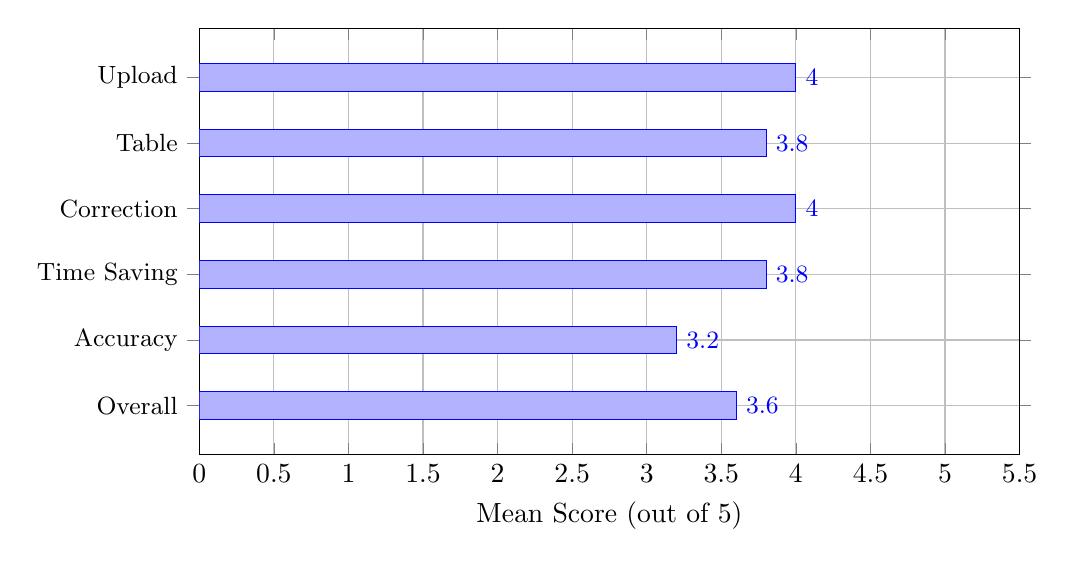
\begin{tikzpicture}
    \begin{axis}[
      xbar, bar width=10pt,
      width=12cm, height=7cm,
      xlabel={Mean Score (out of 5)},
      xmin=0, xmax=5.5,
      symbolic y coords={Overall,Accuracy,Time Saving,Correction,Table,Upload},
      ytick=data,
      yticklabel style={font=\small},
      nodes near coords, nodes near coords style={font=\small},
      enlarge y limits=0.15,
      grid=major,
    ]
    \addplot coordinates {
      (4.00,Upload)(3.80,Table)(4.00,Correction)(3.80,Time Saving)(3.20,Accuracy)(3.60,Overall)
    };
    \end{axis}
  \end{tikzpicture}
  \caption{คะแนนความพึงพอใจของผู้ใช้งานเฉลี่ยในแต่ละเกณฑ์ความสะดวกในการใช้งาน (n=5)}
  \label{fig:usability_bar}
\end{figure}

\subsection{การอภิปรายคะแนนความเชื่อมั่นในความแม่นยำ (3.20/5.00)}

ทั้งนี้ ความล้มเหลวเพียงครั้งเดียวในภารกิจการแก้ไขผลด้วยมือ (Manual correction) ของ U2 เกิดขึ้นเนื่องจาก Interface ต้องการให้ผู้ใช้งานคลิกโดยตรงบนเซลล์ข้อมูลในตาราง ซึ่งไม่ชัดเจนสำหรับผู้ใช้งานที่ไม่คุ้นเคยกับรูปแบบ Spreadsheet บนเว็บ การมีปุ่ม ``Edit'' ที่เด่นชัดกว่านี้จะช่วยแก้ปัญหาด้าน Discoverability ได้ ในส่วนของคะแนนเชิงปริมาณ เกณฑ์ที่ได้คะแนนต่ำที่สุดคือ ``Trust in system accuracy'' (3.20/5.00) คะแนนนี้จำเป็นต้องมีการตีความอย่างระมัดระวัง สำหรับผู้เชี่ยวชาญทางคลินิกที่มีประสบการณ์ (U1 และ U5) ความเชื่อมั่นในความแม่นยำมีความแตกต่างกัน: U5 ให้คะแนน 4 ในขณะที่ U1 ให้คะแนน 3 ซึ่งสะท้อนถึงความกังวลของ U1 ที่ว่าค่า ZOI ที่วัดได้ในบางครั้งแตกต่างจากการกะประมาณด้วยสายตาที่พวกเขาฝึกฝนมามากกว่า 2 mm ซึ่งเป็นระยะที่ส่งผลอย่างมีนัยสำคัญทางคลินิกสำหรับการจัดกลุ่มความไวในกรณีที่อยู่กึ่งกลางขอบเขต (Borderline susceptibility classification) ส่วนผู้เข้าร่วมระดับเริ่มต้นทั้งสองท่านที่เคยทำการทดสอบ Kirby-Bauer ของจริง (ซึ่งไม่มีเลย) ให้คะแนนที่ 2 บ่งชี้ว่าหากไม่มีกรอบอ้างอิงว่าค่าความคลาดเคลื่อนในการวัดระดับใดที่ยอมรับได้ ผู้ใช้งานมักจะตั้งแง่สงสัยไว้ก่อน

ข้อมูลเชิงคุณภาพหลังการทดสอบระบุถึงความคาดหวังที่ยังไม่ได้รับการตอบสนองสองประการ:
\begin{enumerate}
  \item \textbf{การขาดการแสดง Reference breakpoints ในมุมมองผลลัพธ์}
        ผู้ใช้งานคาดหวังว่าระบบจะแสดงค่า CLSI breakpoint (mm) ควบคู่ไปกับค่า ZOI ที่วัดได้ เพื่อให้พวกเขาสามารถตรวจสอบได้ทันทีว่าการจัดกลุ่ม S/I/R แบบอัตโนมัตินั้นสอดคล้องกับขอบเขตเชิงตัวเลขหรือไม่ หากไม่มีบริบทนี้ ผลลัพธ์การจัดกลุ่มจึงถูกรับรู้ว่าเป็นเสมือน ``กล่องดำ (Black box)''
  \item \textbf{ไม่มีตัวบ่งชี้ความเชื่อมั่น (Confidence indicator)}
        ผู้ใช้งานที่มีประสบการณ์ระบุถึงความต้องการคะแนนความเชื่อมั่น (Confidence score) ต่อแต่ละแผ่นยา หรือการแสดงภาพซ้อนทับ (Visual overlay) ที่แสดงขอบเขตของบริเวณยับยั้งที่ตรวจจับได้บนภาพต้นฉบับ เพื่อให้พวกเขาสามารถระบุได้อย่างรวดเร็วว่าการวัดใดที่ควรตรวจสอบด้วยมืออีกครั้ง
\end{enumerate}

การค้นพบเหล่านี้บ่งชี้ว่าปัญหาเรื่องความไม่เชื่อมั่นในความแม่นยำส่วนหนึ่งเป็นปัญหาด้าน \emph{ส่วนต่อประสานกับผู้ใช้งาน (User interface)} มากกว่าที่จะเป็นปัญหาเรื่องความแม่นยำในการวัดเพียงอย่างเดียว การเพิ่มการแสดงผล Breakpoint และมุมมอง Bounding-box overlay ในการพัฒนาครั้งถัดไปมีแนวโน้มที่จะช่วยเพิ่มคะแนนในส่วนนี้ขึ้นได้ 0.5--1.0 คะแนนโดยไม่ต้องมีการเปลี่ยนแปลงใดๆ ใน Pipeline ของ ML

\subsection{สรุปผลการประเมินโดยรวม (Overall Evaluation Summary)}

คะแนนความเป็นประโยชน์โดยรวมที่ 3.60/5.00 นั้นสอดคล้องกับมาตรฐานความสะดวกในการใช้งานที่เผยแพร่สำหรับต้นแบบระบบสนับสนุนการตัดสินใจทางคลินิกรุ่นแรก โดยคะแนนในช่วง 3.4--3.8 ถือเป็นตัวบ่งชี้ว่าระบบมีศักยภาพที่ชัดเจนแต่ยังไม่ถึงระดับที่พร้อมใช้งานจริง (Production readiness) \cite{rajasekar2023} คะแนนในส่วน Upload workflow (4.00) และ Manual correction (4.00) ยืนยันว่าการออกแบบการปฏิสัมพันธ์หลักนั้นมีประสิทธิภาพ ความแตกต่างระหว่างคะแนน Workflow ที่สูงและคะแนนความเชื่อมั่นในความแม่นยำที่ต่ำกว่าชี้ให้เห็นอย่างชัดเจนว่าการแสดงผลความแม่นยำเป็นพื้นที่หลักสำหรับการปรับปรุง

อย่างไรก็ตาม เป็นสิ่งสำคัญที่ต้องระบุว่าการประเมินความพึงพอใจผู้ใช้งานในการศึกษานี้ดำเนินการในลักษณะของ \textbf{การประเมินเบื้องต้นแบบ Pilot ที่มีจำนวนผู้เข้าร่วมจำกัด} (The usability evaluation was conducted as a preliminary pilot assessment with a limited number of participants.) ผลลัพธ์ที่ได้จากผู้เข้าร่วม 5 ท่านยังไม่สามารถใช้เป็นตัวแทนของประชากรผู้ใช้งานในวงกว้างได้ทางสถิติ การศึกษาความพึงพอใจผู้ใช้งานในระดับที่ใหญ่กว่า ครอบคลุมบุคลากรห้องปฏิบัติการจากหลายสถาบันและหลายภูมิภาค จะเป็นสิ่งจำเป็นสำหรับการยืนยันที่มีนัยสำคัญยิ่งขึ้น (A larger-scale user study involving multiple laboratory personnel is required for stronger validation.)

ข้อมูลเชิงคุณภาพที่รวบรวมจากผู้เข้าร่วมยังให้ Feedback ที่มีคุณค่าสำหรับการพัฒนาในอนาคต ได้แก่: ผู้ใช้งานพบว่าฟังก์ชันการแก้ไขผลลัพธ์ OCR มีประโยชน์อย่างมากในการแก้ไขข้อผิดพลาดที่ระบบตรวจจับไม่ถูกต้อง; มีการร้องขอ Workflow การอัปโหลดที่รวดเร็วกว่านี้ โดยเฉพาะสำหรับการประมวลผลภาพหลายภาพพร้อมกัน; และผู้เชี่ยวชาญทางคลินิกแสดงความกังวลเกี่ยวกับกรณี Borderline zones ที่ค่า ZOI ใกล้เคียงกับจุดตัดของ Breakpoint ซึ่งต้องการความแม่นยำสูงเป็นพิเศษ

% ─────────────────────────────────────────────────────────────
\section{เว็บแอปพลิเคชัน (Web Application)}
\label{sec:webapp}
% ─────────────────────────────────────────────────────────────

React frontend ได้รับการพัฒนาจนเสร็จสมบูรณ์ โดยมีส่วนต่อประสานที่ใช้งานง่ายสำหรับการอัปโหลดภาพ การจับภาพสดจากกล้อง และการแสดงผลลัพธ์ที่เป็นภาพรวม ซึ่งรวมถึง Dashboard ที่แสดงเส้นผ่านศูนย์กลาง ZOI และการจัดกลุ่ม S/I/R ต่อชนิดยาปฏิชีวนะ ส่วนต่อประสานรองรับทั้งการใช้งานบน Desktop และ Tablet ซึ่งเหมาะสมสำหรับการติดตั้งใช้งาน ณ จุดดูแลผู้ป่วย (Point-of-care) บนสถานีงานในห้องปฏิบัติการที่ใช้ร่วมกัน

ส่วนของ Backend REST API (FastAPI) และการบูรณาการฐานข้อมูล PostgreSQL อยู่ในขั้นตอนต้นแบบขั้นสูง โดยมี Endpoint สำหรับการส่งภาพ การเรียกข้อมูลผลลัพธ์ และการส่งออกรายงานที่ได้รับการพัฒนาและทดสอบแยกส่วนแล้ว การทดสอบระบบแบบ End-to-end อย่างเต็มรูปแบบ ซึ่งรวมทั้ง Frontend, Backend, Model inference server และฐานข้อมูลในสภาพแวดล้อมที่เทียบเท่ากับการใช้งานจริง ถือเป็นเป้าหมายหลักที่เหลืออยู่เพื่อให้ระบบมีความพร้อมในการปฏิบัติงานอย่างสมบูรณ์

\begin{figure}[H]
  \centering
  \safeimg[width=0.9\textwidth]{figures/webapp_screenshot.png}{Web application dashboard screenshot}
  \caption{หน้าจอ Dashboard ของระบบ ZoneAnalyzer แสดงผลการวัด ZOI และการจัดกลุ่ม S/I/R}
  \label{fig:webapp}
\end{figure}

\begin{figure}[H]
  \centering
  \safeimg[width=0.82\textwidth]{figures/_review/webapp_03_upload.png}{ZoneAnalyzer upload page}
  \caption{หน้าอัปโหลดภาพของระบบ ZoneAnalyzer}
  \label{fig:webapp_upload}
\end{figure}

\begin{figure}[H]
  \centering
  \safeimg[width=0.82\textwidth]{figures/_review/webapp_01_home_landing.png}{ZoneAnalyzer landing page}
  \caption{หน้าแรก (Landing page) ของระบบ ZoneAnalyzer}
  \label{fig:webapp_home}
\end{figure}
